\section{The Problem}
 \begin{wrapfigure}{r}{0.30\columnwidth}
\vspace{-3em}
		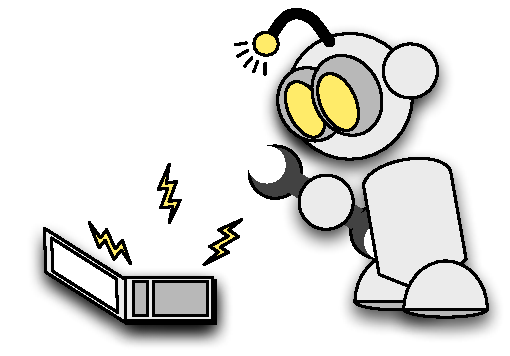
\includegraphics[width=0.30\columnwidth]{diagrams/robot_mechanic.pdf}
 \end{wrapfigure}

Pathfinding in modern video games often involves exploring \textbf{highly regular 
environments} such as cities, sewers or dungeons -- see for example
Figure \ref{fig:iw2}.
These locations are usually symmetric in the sense that many optimal 
length paths exist between arbitrary pairs of locations.
\textbf{Symmetry is undesirable} as it increases the size of the search space and forces
search algorithms to waste time.
\newline \newline
In this work we \textbf{speed up pathfinding} by identifying and eliminating
symmetry \textbf{in 4-connected grid maps}.
Our method is fast, optimal, memory efficient and readily combined with any
existing pathfinding system.
\vspace{1em}
 \begin{figure}[h]
  \centering
  \begin{minipage}{0.47\columnwidth}
	\label{fig:wc3}
	\centering
		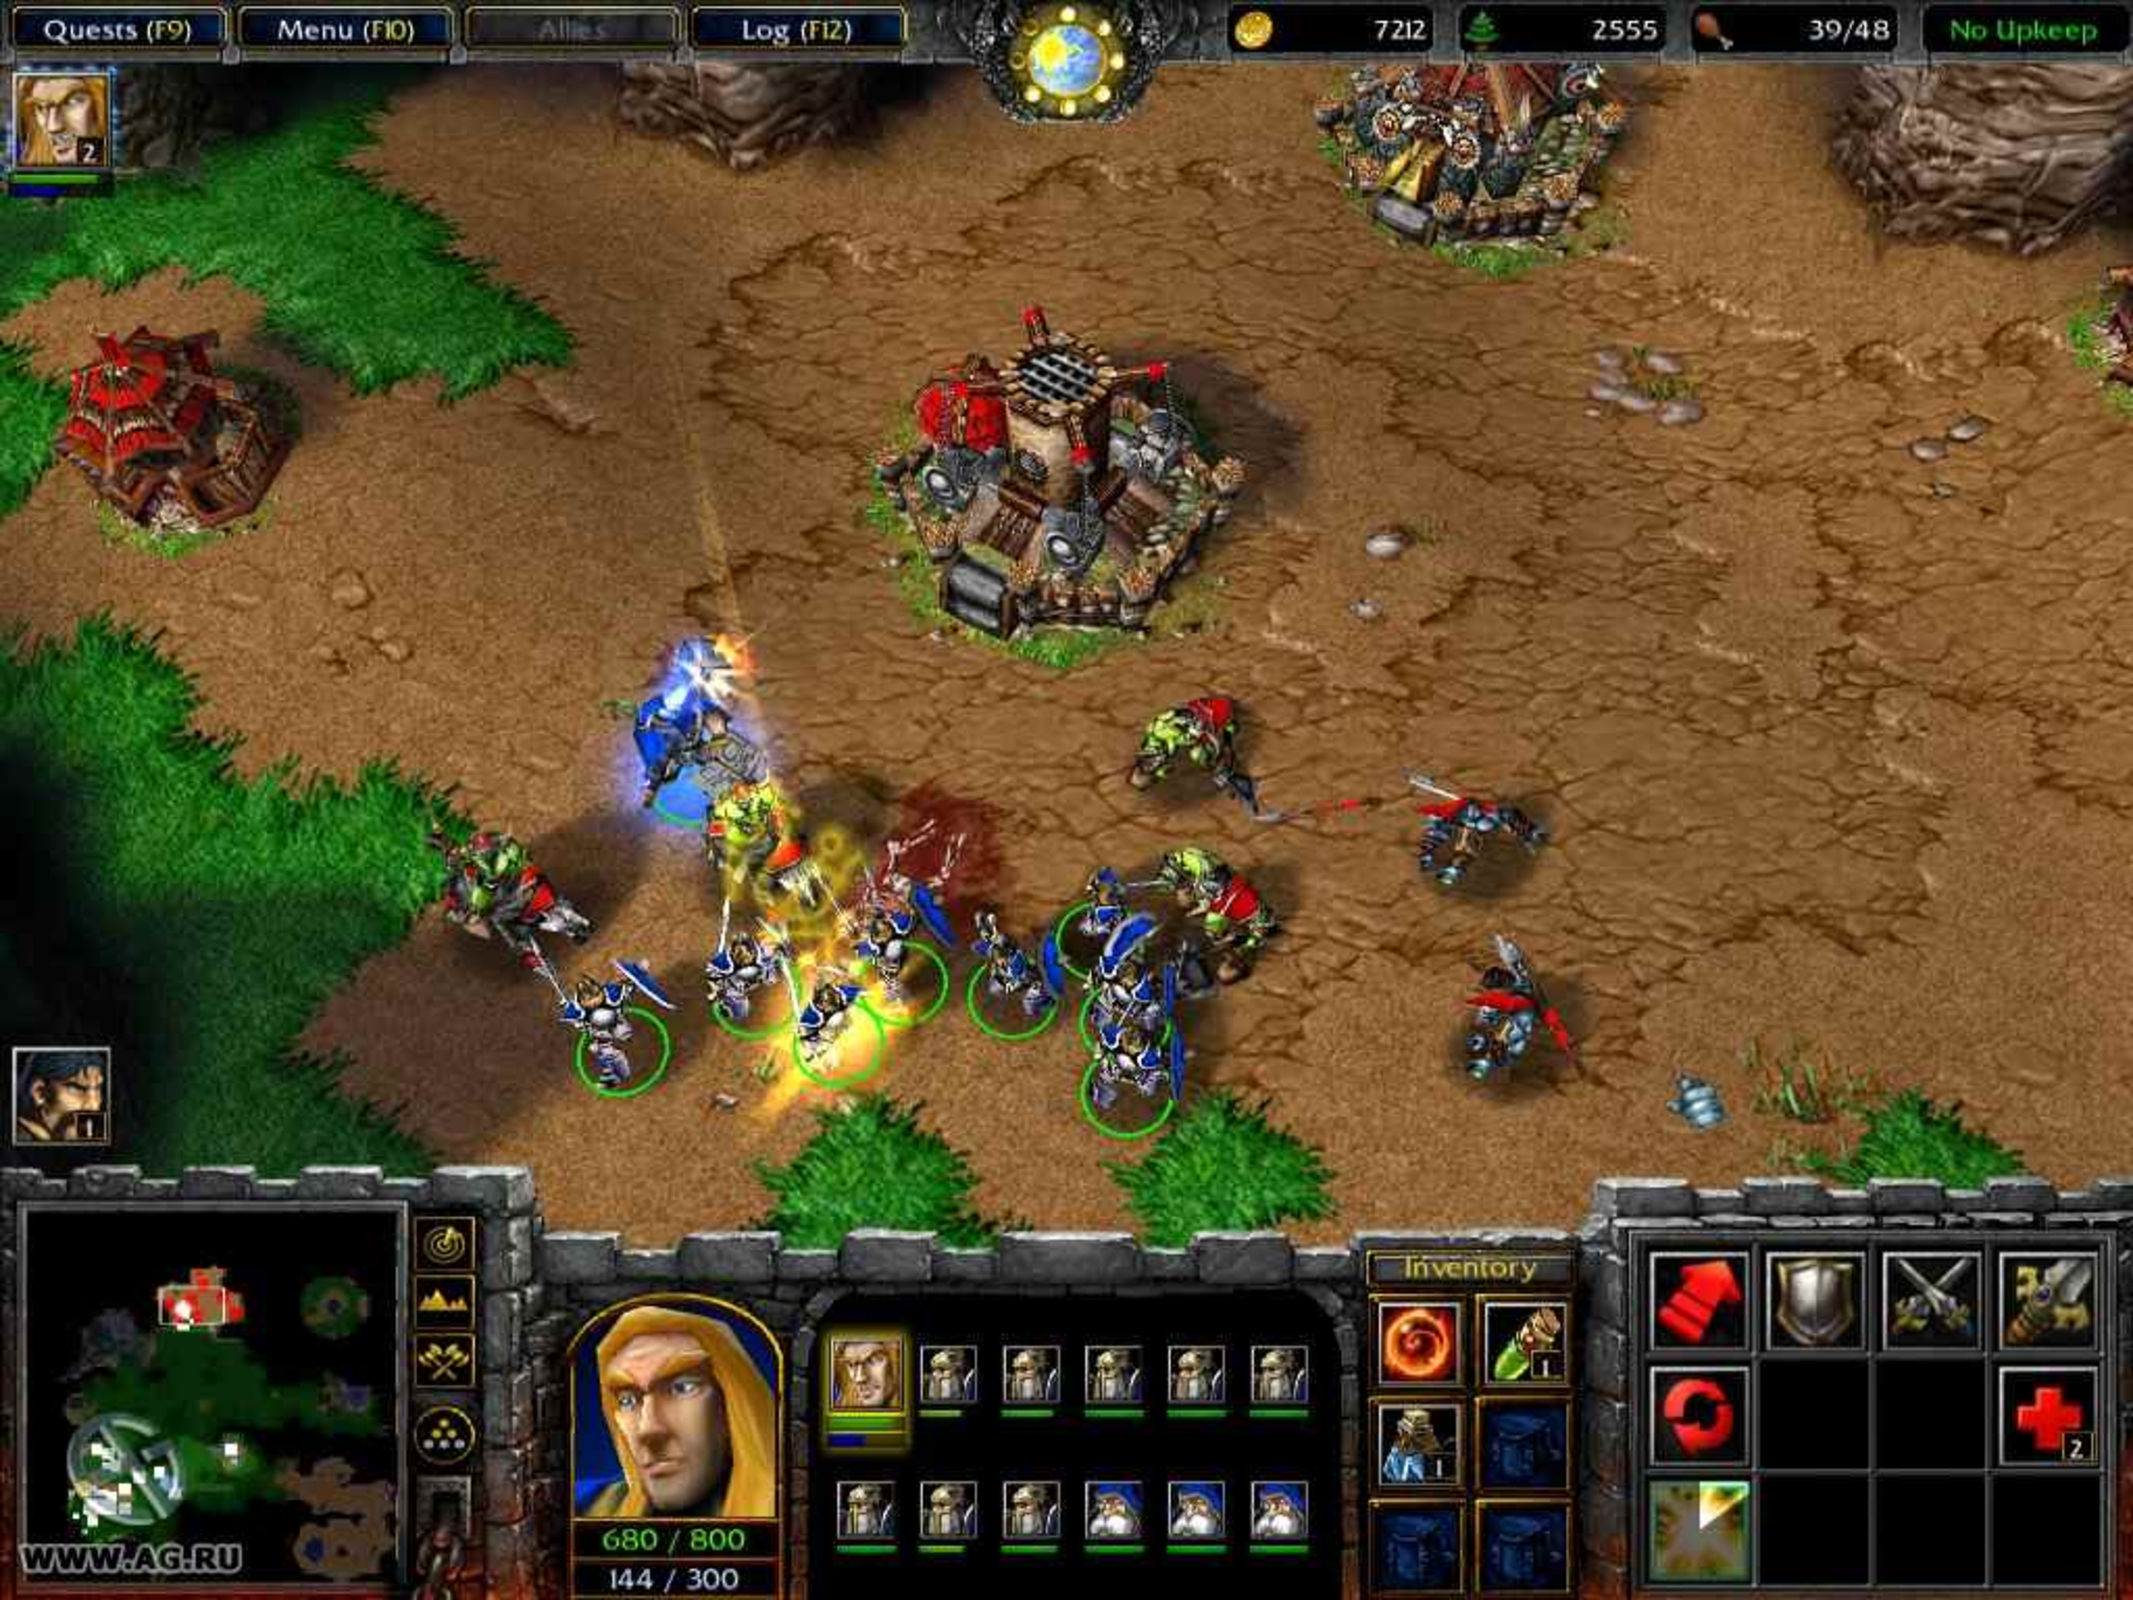
\includegraphics[width=\columnwidth]{diagrams/wc3.pdf}
	\end{minipage}
  \hspace{0.35em}
  \begin{minipage}{0.47\columnwidth}
	\label{fig:iw2}
	\centering
		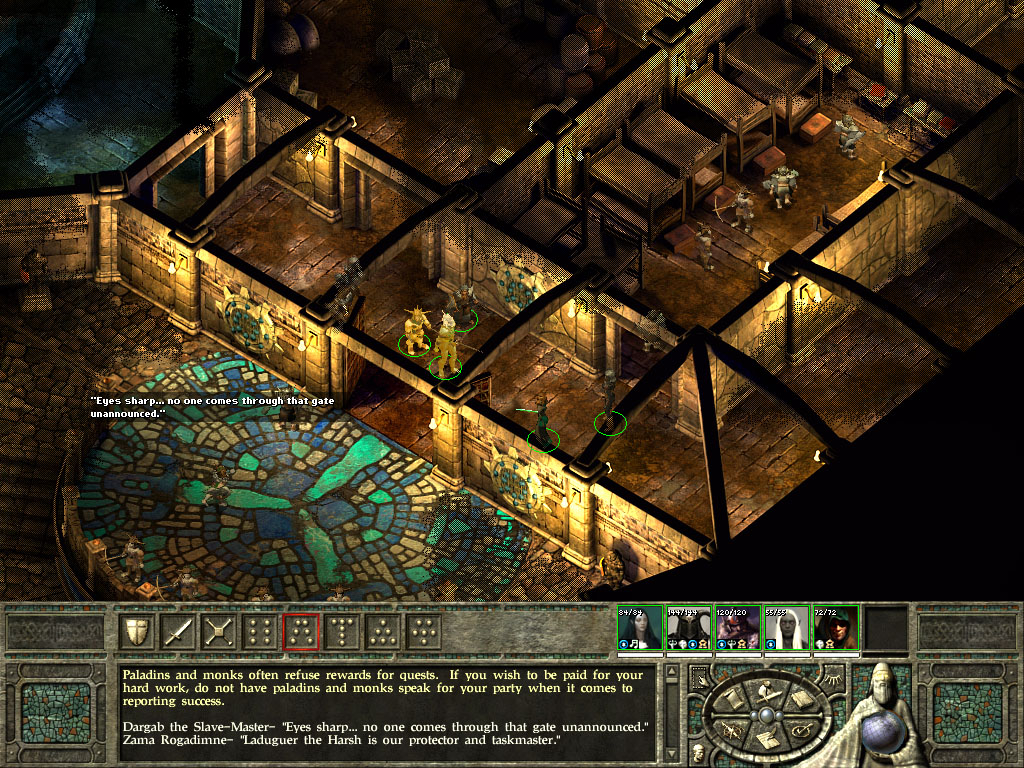
\includegraphics[width=\columnwidth]{diagrams/iwdale.jpg}
	\end{minipage}
\end{figure}
\begin{figure}[h]
   \centering
    \begin{minipage}{0.47\columnwidth}
		\label{fig:ra3}
		\centering
			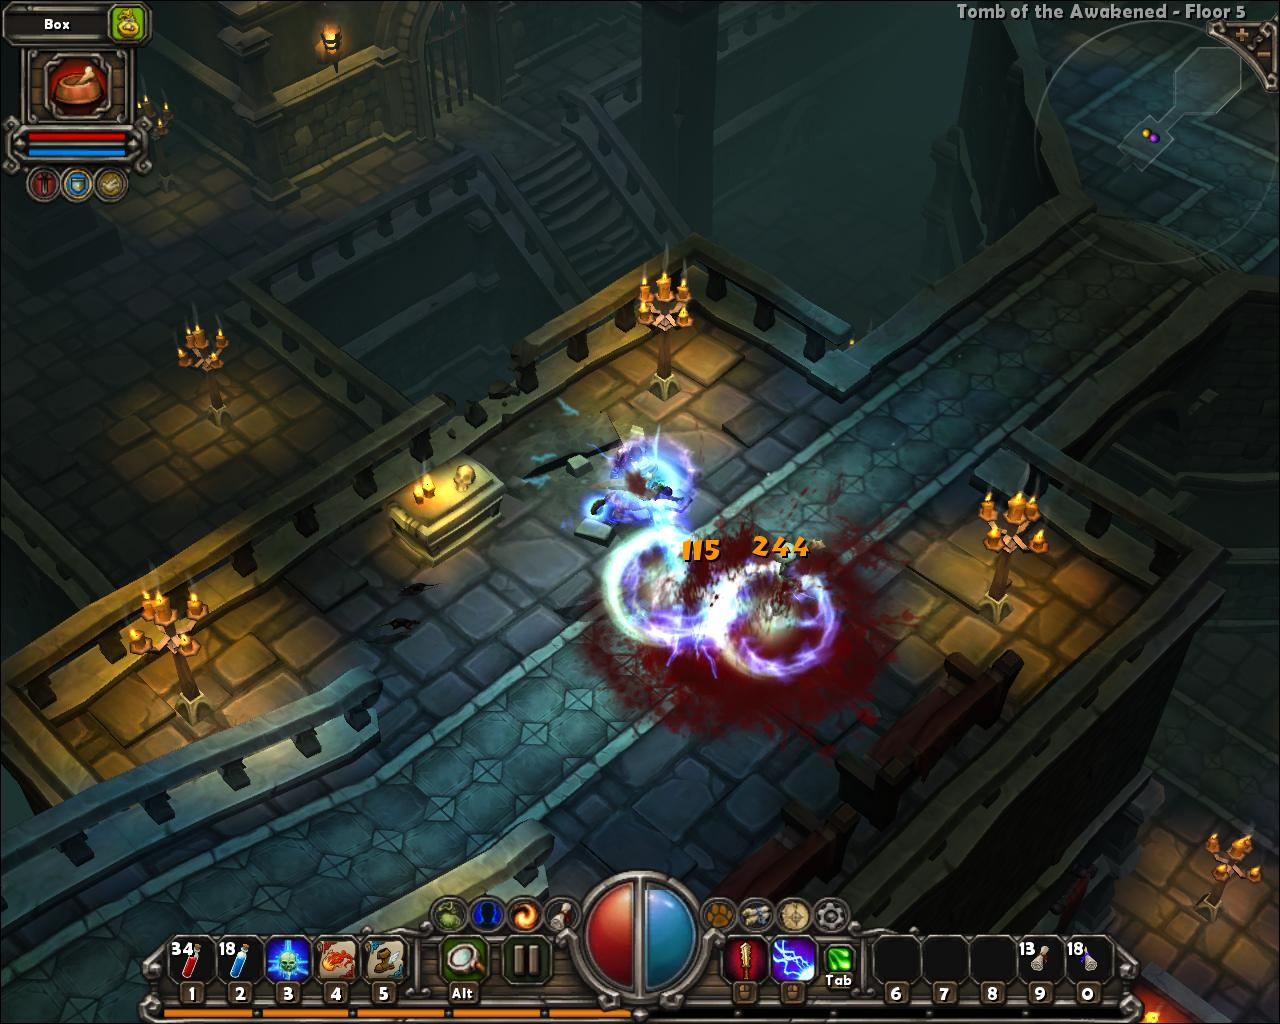
\includegraphics[width=\columnwidth]{diagrams/torchlight.jpg}
	\end{minipage}
  \hspace{0.35em}
    \begin{minipage}{0.47\columnwidth}
		\label{fig:ra3u}
		\centering
			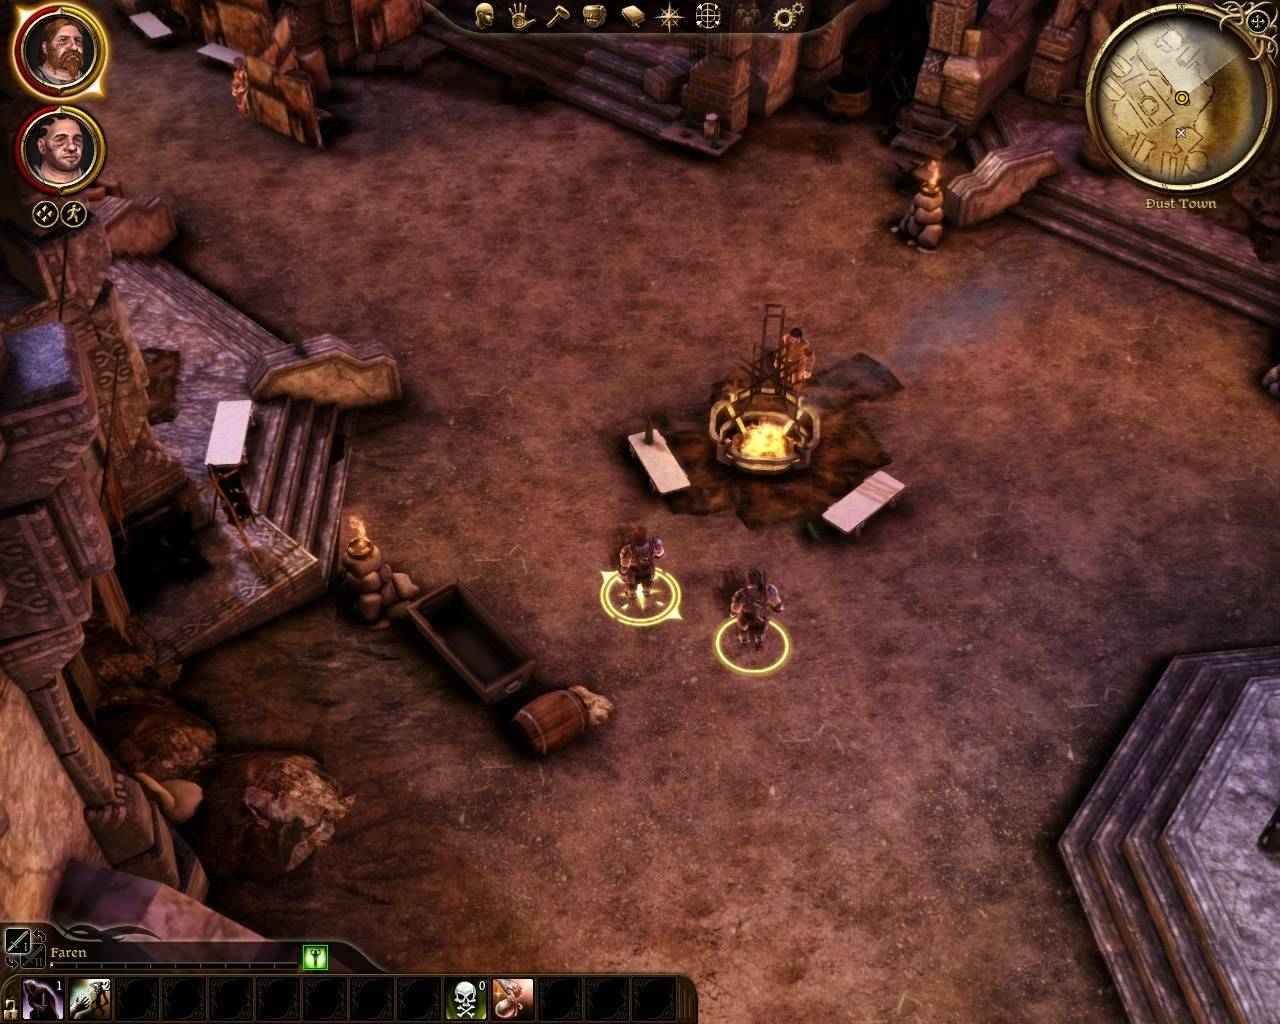
\includegraphics[width=\columnwidth]{diagrams/da.jpg}
	\end{minipage}
\caption{Typical examples of highly regular video game environments.}

 \end{figure}

